\section{Introduction}

\begin{wrapfigure}{r}{4.1cm}
\caption{Joseph Fourier (1768-1830).}\label{wrap-fig:1}
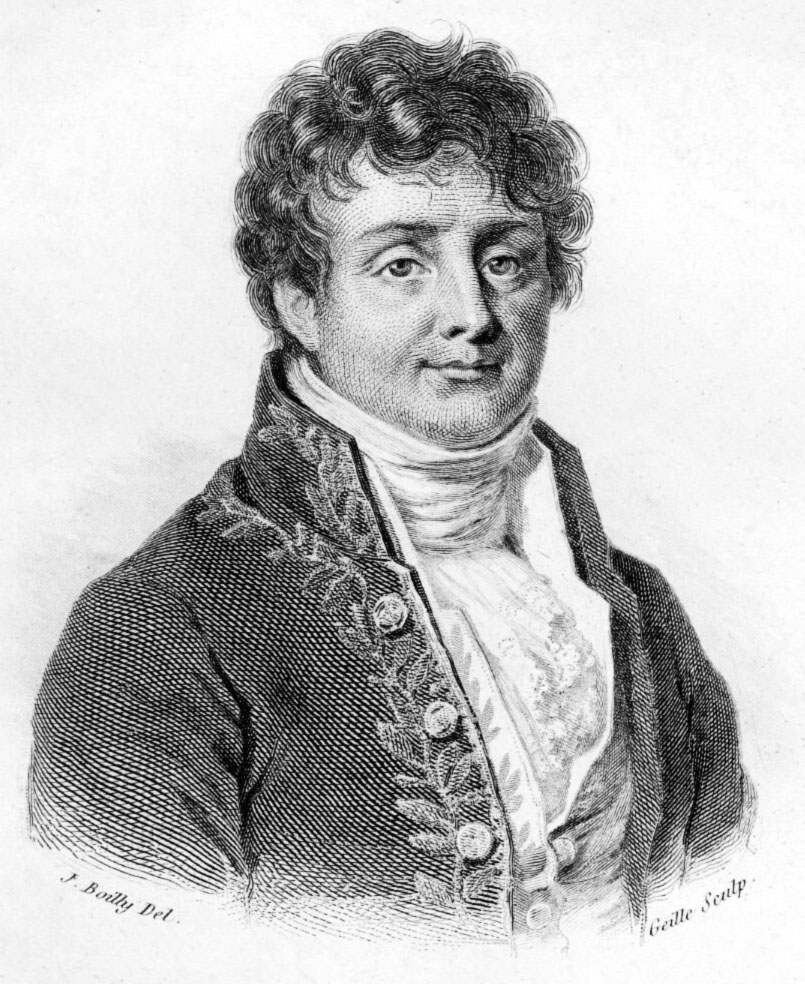
\includegraphics[width=4cm]{images/joseph_fourier.jpg}
\end{wrapfigure}

Au début du XIX\textsuperscript{ème}, le mathématicien Joseph Fourier travaille à la résolution de l'équation de la chaleur \cite{wiki-chaleur} , une équation aux dérivées partielles modélisant le phénomène de conduction thermique.
Dans le cadre de ses travaux, il introduit la notion de séries de Fourier, un développement en série trigonométrique des fonctions périodiques, et plus généralement la transformée de Fourier. Ces deux concepts seront alors étudiés minutieusement et donneront lieu à d'importantes découvertes en mathématiques, physique et informatique.

Le présent document aura pour objectif de formaliser la transformée de Fourier dans le cadre de la théorie du traitement du signal afin de comprendre comment cet outil peut être exploité en informatique pour la compression d'images numériques et de signaux sonores. On s'attardera en particulier sur l'implémentation et les applications de l'algorithme FFT (\og Fast Fourier Transform \fg pour transformée de Fourier rapide) permettant de calculer très efficacement des transformées de Fourier.